\documentclass{report}
\usepackage[utf8]{inputenc}
\usepackage[spanish]{babel}
\usepackage[margin=2cm]{geometry}
\usepackage{graphicx}
\usepackage{float}
\usepackage{titlesec}
\usepackage{caption}
\usepackage{listings}
\usepackage{xcolor}
\usepackage{array}
\usepackage{booktabs}
\usepackage{tabularx} 
\usepackage{multirow}
\usepackage{amsmath}
\usepackage{hyperref}

\definecolor{codegreen}{rgb}{0,0.6,0}
\definecolor{codegray}{rgb}{0.5,0.5,0.5}
\definecolor{codepurple}{rgb}{0.58,0,0.82}
\definecolor{backcolor}{rgb}{0.95,0.95,0.95}


\lstset{
    basicstyle=\ttfamily,
    inputencoding=utf8,
    extendedchars=true,
    literate=%
    {á}{{\'a}}1
    {é}{{\'e}}1
    {í}{{\'i}}1
    {ó}{{\'o}}1
    {ú}{{\'u}}1
    {ñ}{{\~n}}1
    {Á}{{\'A}}1
    {É}{{\'E}}1
    {Í}{{\'I}}1
    {Ó}{{\'O}}1
    {Ú}{{\'U}}1
    {Ñ}{{\~N}}1
}


\lstdefinestyle{mystyle}{
    backgroundcolor=\color{backcolor},
    commentstyle=\color{codegreen},
    keywordstyle=\color{red},
    numberstyle=\tiny\color{codegray},
    stringstyle=\color{codepurple},
    basicstyle=\ttfamily\footnotesize,
    breakatwhitespace=false,
    breaklines=true,
    captionpos=b,
    keepspaces=true,
    numbers=left,
    showspaces=false,
    showstringspaces=false,
    showtabs=false,
    tabsize=2  
}

\titleformat{\section}
{\huge\bfseries}{\thesection.}{1em}{}
\titleformat{\subsection}
{\large\bfseries}{\thesubsection}{1em}{}

\renewcommand\thesection{\arabic{section}}

\title{\Huge{\textbf{Practica 5. Optimización por Colonia de Hormigas}}\\
\Large{\textbf{Algoritmos Bioinspirados}}}
\author{Diego Castillo Reyes\\Marthon Leobardo Yañez Martinez\\Aldo Escamilla Resendiz}

\graphicspath{{imagenes/}}

\begin{document}
\maketitle
\tableofcontents
\section{Introducción}
El Algoritmo de Optimización por Colonia de Hormigas (ACO, por sus siglas en inglés) es una técnica metaheurística inspirada en el comportamiento de las hormigas en la naturaleza. Este algoritmo, propuesto inicialmente por Marco Dorigo en la década de 1990, simula la forma en que las hormigas encuentran caminos óptimos entre su colonia y una fuente de alimento.

En la naturaleza, las hormigas depositan feromonas en su camino al buscar comida, creando un rastro químico que guía a otras hormigas. Con el tiempo, los caminos con más feromonas se vuelven más atractivos, y las hormigas tienden a seguir estos senderos más prometedores, lo que eventualmente conduce a la convergencia en el camino más corto.

El ACO utiliza este principio para resolver problemas de optimización combinatoria. En este algoritmo, una colonia de hormigas artificiales construye soluciones al problema, y durante este proceso, cada hormiga deposita feromonas en el entorno, influyendo en las decisiones de las hormigas subsiguientes. Los caminos que resultan en mejores soluciones reciben más feromonas, aumentando la probabilidad de ser seleccionados en iteraciones futuras.

\section{Problema de Asignación Cuadrática}
\lstinputlisting[language=Python, style=mystyle]{ACO.py}
\begin{figure}[H]
    \centering
    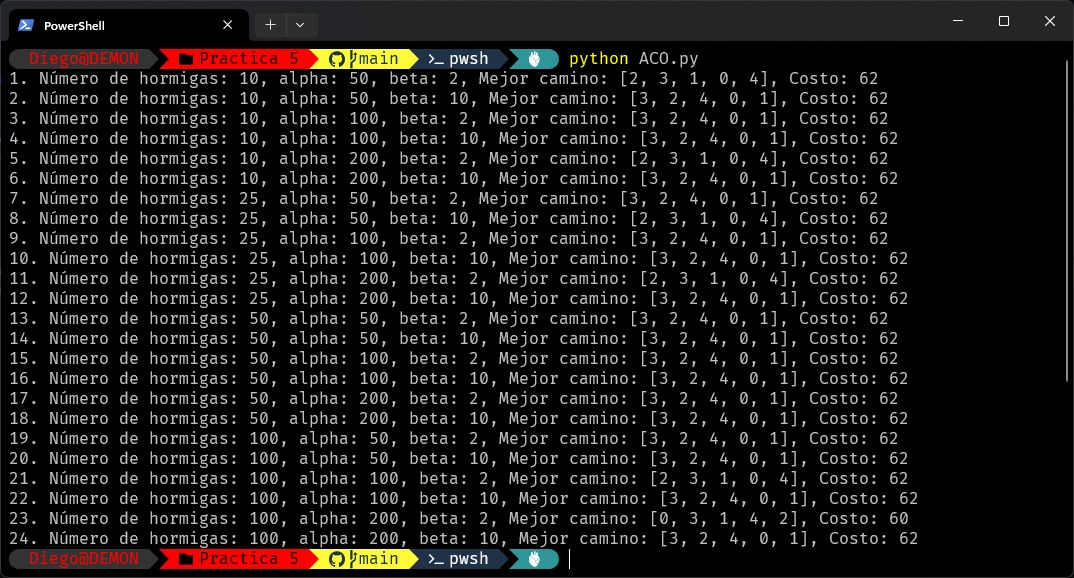
\includegraphics[width=0.8\textwidth]{ajuste.dat.jpeg}
    \caption{Pruebas de regresión}
    \label{fig:prueba matriz}
\end{figure}
\begin{figure}[H]
    \centering
    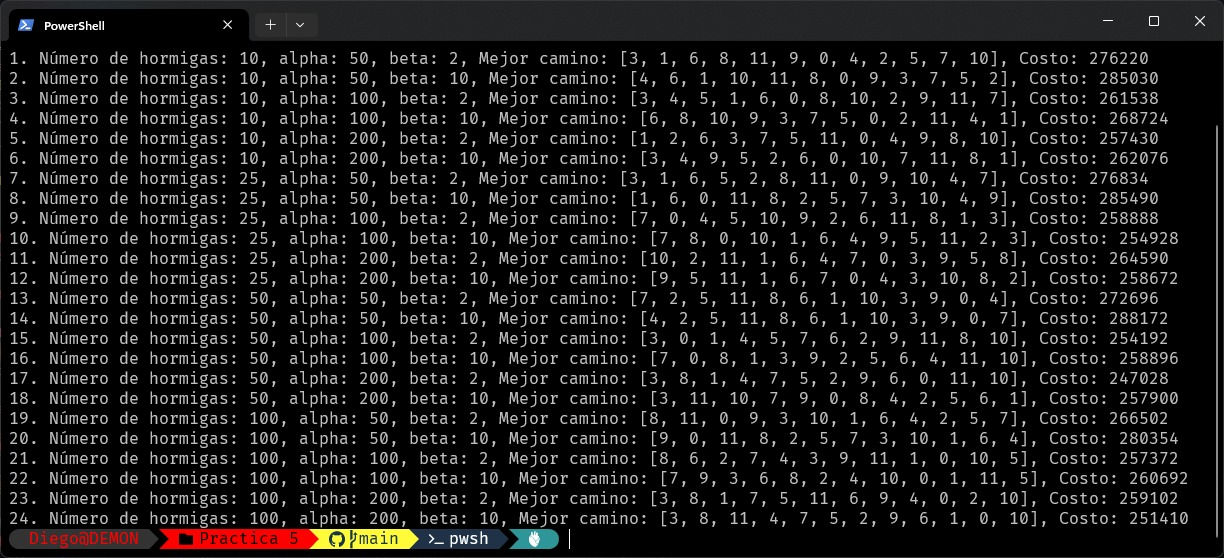
\includegraphics[width=0.8\textwidth]{tai12.dat.jpeg}
    \caption{Pruebas de regresión}
    \label{fig:prueba tai12}
\end{figure}
\begin{figure}[H]
    \centering
    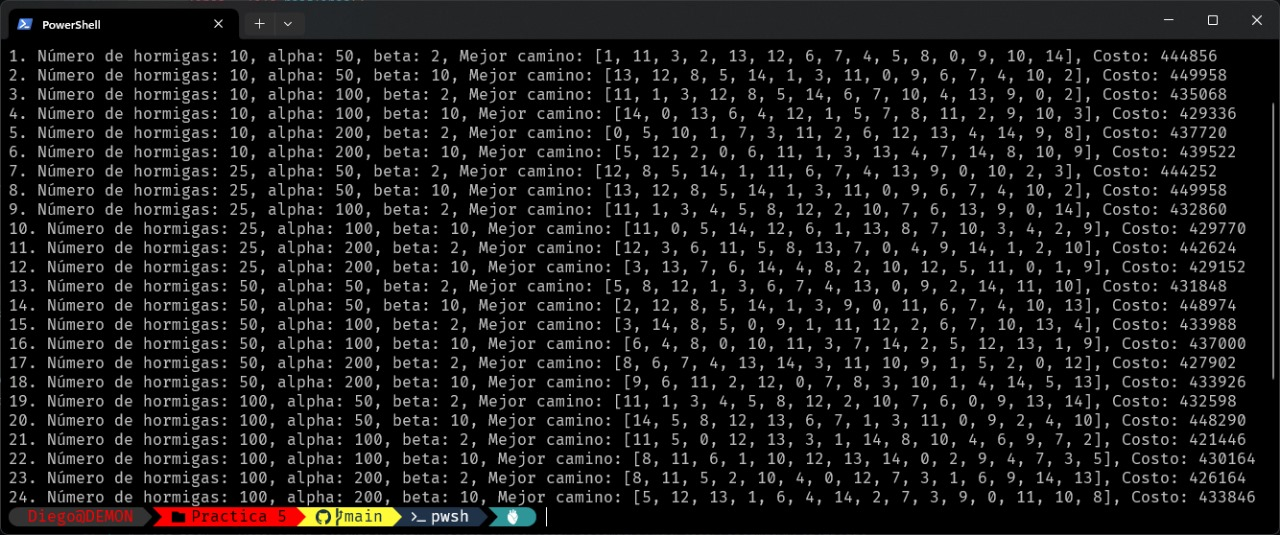
\includegraphics[width=0.8\textwidth]{tai15.dat.jpeg}
    \caption{Pruebas de regresión}
    \label{fig:prueba tai15}
\end{figure}
\begin{figure}[H]
    \centering
    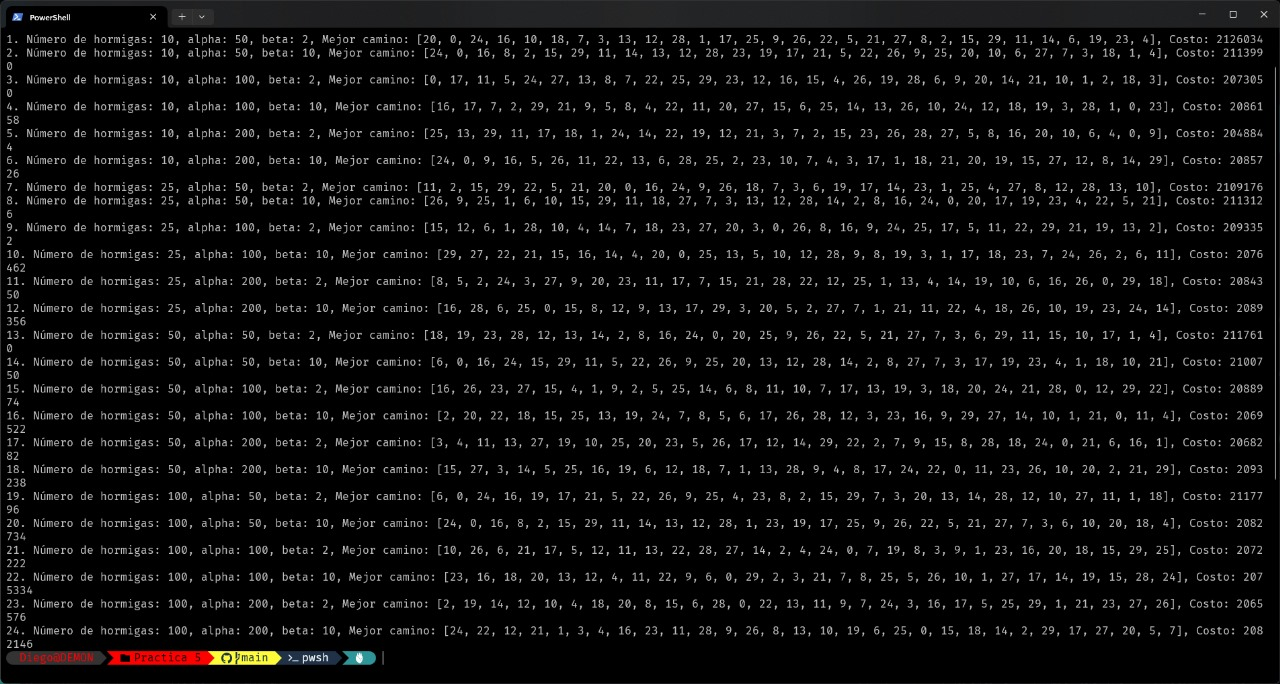
\includegraphics[width=0.8\textwidth]{tai30.dat.jpeg}
    \caption{Pruebas de regresión}
    \label{fig:prueba tai30}
\end{figure}
\section{Lectura}
Problema de Optimización Combinatoria Resuelto por ACO

El Algoritmo de Optimización por Colonia de Hormigas (ACO) resuelve problemas de optimización combinatoria convirtiéndolos en problemas de encontrar el camino más corto en un grafo ponderado. Formalmente, esto se describe como:

\begin{itemize}
    \item \textbf{Grafo Ponderado} \(G = (V, E)\): donde \(V\) es el conjunto de vértices y \(E\) es el conjunto de aristas.
    \item \textbf{Función de Costo} \(c: E \rightarrow \mathbb{R}^+\): Asigna un costo positivo a cada arista.
    \item \textbf{Soluciones} \(S\): Conjuntos de caminos en el grafo.
    \item \textbf{Función Objetivo} \(f: S \rightarrow \mathbb{R}\): Evaluación del costo de cada solución.
\end{itemize}

Las hormigas artificiales construyen soluciones explorando el grafo, guiadas por niveles de feromonas que reflejan la calidad de soluciones previas.

Cuadro Comparativo de Versiones de ACO

\begin{table}[h!]
\centering
\begin{tabular}{|c|p{10cm}|}
\hline
\textbf{Versión ACO} & \textbf{Descripción} \\
\hline
\textbf{Ant System (AS)} & Primera versión básica de ACO. Las hormigas depositan feromonas proporcionalmente a la calidad de la solución encontrada. \\
\hline
\textbf{Ant Colony System (ACS)} & Introduce la actualización local de feromonas y un mecanismo de exploración más agresivo para evitar la convergencia prematura. \\
\hline
\textbf{Max-Min Ant System (MMAS)} & Establece límites máximo y mínimo a los niveles de feromonas, ayudando a prevenir la convergencia en soluciones subóptimas. \\
\hline
\textbf{Rank-Based Ant System (RAS)} & Asigna diferentes cantidades de feromonas según el ranking de las soluciones, favoreciendo las mejores soluciones encontradas. \\
\hline
\textbf{Elitist Ant System (EAS)} & Similar a AS, pero con un sesgo adicional hacia las mejores soluciones almacenadas en una memoria global. \\
\hline
\textbf{Hybrid Ant System (HAS)} & Combina ACO con otros métodos de optimización como el recocido simulado o algoritmos genéticos para mejorar la exploración y explotación del espacio de soluciones. \\
\hline
\end{tabular}
\caption{Comparación de versiones de ACO}
\end{table}

El último congreso registrado es el "ANTS 2022 - International Conference on Swarm Intelligence". Los tópicos abordados incluyeron:

\begin{itemize}
    \item Algoritmos bioinspirados
    \item Optimización multiobjetivo
    \item Aplicaciones industriales de ACO
    \item Modelado y análisis teórico de ACO
\end{itemize}

Las pláticas cubrieron avances recientes en teoría de feromonas, aplicaciones prácticas y nuevas variantes híbridas del algoritmo.

Aplicaciones Relevantes

\begin{table}[H]
\centering
\begin{tabular}{|c|p{10cm}|}
\hline
\textbf{Tipo de Aplicación} & \textbf{Descripción} \\
\hline
\textbf{Mono-objetivo} & Resolución del problema del viajero, optimización de rutas en redes de telecomunicaciones, y diseño de circuitos electrónicos. \\
\hline
\textbf{Multiobjetivo} & Optimización de problemas de programación de la producción, planificación de horarios en universidades, y diseño de redes robustas. \\
\hline
\end{tabular}
\caption{Aplicaciones Relevantes de ACO}
\end{table}
\section{Conclusiones}
Escamilla Resendiz Aldo:
El algoritmo de optimización por colonia de hormigas es una técnica metaheurística que ha demostrado ser efectiva en la resolución de problemas de optimización combinatoria. A través de la simulación del comportamiento de las hormigas en la naturaleza, el ACO es capaz de encontrar soluciones de alta calidad en un tiempo razonable. Las diferentes versiones de ACO ofrecen una variedad de enfoques para abordar problemas específicos, y su flexibilidad permite adaptarse a una amplia gama de aplicaciones.
En el contexto de la configuración de parámetros, ANOVA ayuda a identificar cuáles parámetros tienen un efecto significativo en el rendimiento del sistema o proceso bajo estudio. Esto se realiza dividiendo la variabilidad total de los datos en componentes atribuibles a diferentes fuentes de variación.\\
\\Yañez Martinez Marthon Leobardo:
El ACO es una técnica de optimización poderosa que ha demostrado ser efectiva en una variedad de aplicaciones. Al simular el comportamiento de las hormigas en la naturaleza, el ACO es capaz de encontrar soluciones de alta calidad para problemas de optimización combinatoria. Las diferentes versiones de ACO ofrecen una variedad de enfoques para abordar problemas específicos, y su flexibilidad permite adaptarse a una amplia gama de aplicaciones.\\
\\Castillo Reyes Diego:
El algoritmo de optimización por colonia de hormigas es una técnica metaheurística que ha demostrado ser efectiva en la resolución de problemas de optimización combinatoria. A través de la simulación del comportamiento de las hormigas en la naturaleza, el ACO es capaz de encontrar soluciones de alta calidad en un tiempo razonable. Las diferentes versiones de ACO ofrecen una variedad de enfoques para abordar problemas específicos, y su flexibilidad permite adaptarse a una amplia gama de aplicaciones.
\end{document}